% Document props and library inclusions
\documentclass[10pt,a4paper]{report} 
\usepackage[utf8]{inputenc} 
\usepackage[swedish]{babel}
\usepackage{mathtools,tikz,textcomp,fixltx2e,color,fullpage,graphicx,afterpage,float,parskip,xfrac,gensymb,titlesec,etoolbox,pdfpages,hyperref}
\usetikzlibrary{calc,matrix,positioning,arrows,shapes,trees,plotmarks,decorations.markings}
\usepackage[font={small,it}]{caption}
\usepackage[europeancurrents,europeanvoltages,europeanresistors,europeaninductors,smartlabels]{circuitikz}
\usepackage[font={small,it}]{caption} %% Italics in captions

\setcounter{secnumdepth}{0} % Levels enumerated

% PDF props
\hypersetup{
  bookmarks=true,              % show bookmarks bar?
  bookmarkstype=toc,
  bookmarksopenlevel=\maxdimen
  unicode=true,                % non-Latin characters in Acrobat’s bookmarks
  pdftoolbar=true,             % show Acrobat’s toolbar?
  pdfmenubar=true,             % show Acrobat’s menu?
  pdffitwindow=false,          % window fit to page when opened
  pdfstartview={FitH},         % fits the width of the page to the window
  pdftitle={Kravspec},         % title
  pdfauthor={Petersson, Oscar}, % author
  pdfsubject={TDDI02},          % subject of the document
  pdfkeywords={TDDI02}          % list of keywords
  pdfnewwindow=true,           % links in new window
  hidelinks,                   % hide links (removing color and border)
  linktocpage=true,
  linktoc=all,                 % parts of TOC made into links
  pdfdisplaydoctitle=true      %display document title instead of file name in title bar
}
\urlstyle{same}

%% First Page Information
\author{Matteus Laurent, Johan Levinsson, Oscar Petersson, Erik Peyronsson}
\title{MatLabb}
\date{\today}
\newcommand{\course}{Programmeringsprojekt, HT15}
\newcommand{\coursenumber}{TDDI02, Linköpings universitet}
\newcommand{\programme}{Högskoleingenjörsutbildning i datateknik, 180 hp}
\newcommand{\examiner}{Johan Frimodig}
\newcommand{\institution}{Institutionen för datavetenskap}
\newcommand{\reptype}{Kravspecifikation}

\newcommand{\includelogo}{
\includegraphics[width=48 mm]{LiTH_sigill_sv.pdf}\makeatletter\begin{center}\vskip 4.5cm}
\newcommand{\excludelogo}{\makeatletter\begin{center}~\vfill}

\begin{document}

\pagestyle{empty}
%\includelogo
 \excludelogo
  \Large{\@author}\vskip .3cm
  \textbf{\LARGE{\@title}}\vskip .2cm
  \large{\programme}
  \vfill
\end{center}
\reptype{} - \@date\hfill Handledare:\\
\textbf{\course}\hfill\examiner\\
\coursenumber\hfill\institution
\makeatother
\newpage

%% Table of Contents
%\addtocontents{toc}{\protect\hypertarget{toc}{}}
%\tableofcontents\label{sec:toc}
%\addtocontents{toc}{\protect\thispagestyle{empty}}
%\cleardoublepage

\section{Bakgrund}
Projektets syfte är att skapa en interaktiv receptdatabas med grafiskt användargränssnitt för att hjälpa användaren med organisering av recept med smarta sökfunktioner och för att underlätta matlagningsprocessen genom att tillåta portions- och enhetsomvandling. För att hjälpa användaren att hålla koll på både sin vikt och ekonomi kommer recepten även innehålla information om näringsinnehåll och pris.

MatLabb måste erbjuda något utöver det som står att finna i normala kokböcker. Att hitta recept i en kokbok kan vara klurigt eftersom att man begränsas till kokbokens index. Man kan exempelvis slå upp 'köttfärs' och få en lista med köttfärsbaserade rätter, men då finner man även rätter som innehåller ingredienser som man inte har tillgång till, rätter som tar längre tid än man har och rätter som på andra sätt faller utanför aktuella ramar. Därför vill vi kunna söka och finna recept på ett mer dynamiskt sätt.


\section{Krav}
\renewcommand{\labelenumii}{\theenumii}
\renewcommand{\theenumii}{\theenumi.\arabic{enumii}.}

\begin{enumerate}
\item Varje recept skall innehålla information om:
  \begin{enumerate}
    \item Titel
    \item En lista över ingredienser samt åtgång av dessa
    \item Portionspris
    \item Energiinnehåll
    \item En beskrivning av tillagningsproceduren
    \item Betyg
  \end{enumerate}
\item Användaren skall via gränsnittet kunna läsa ett valt recepts ingredienser, tillagningsprocedur samt betyg.
\item Användaren skall kunna lägga in egna recept i databasen via gränssnittet genom att välja vilka ingredienser som ingår, ange mängd samt skriva en beskrivning.
\item Användaren skall kunna lägga till nya ingredienser i databasen via gränssnittet genom att ange namn, pris samt energiinnehåll.
\item Användaren skall kunna justera pris och energiinnehåll hos en ingrediens via gränssnittet
\item Användaren skall med hjälp av gränssnittet kunna ändra ett recepts betyg på en femgradig skala
\item Recept skall med hjälp av gränsnittet kunna filtreras med hjälp av följande filter:
  \begin{enumerate}
    \item Titel
    \item Ingående ingredienser
    \item Kostnad
    \item Energiinnehåll
    \item Allergier
    \item Vegetarisk
  \end{enumerate}
\item Användaren skall kunna skala om ett recept till valt antal portioner
\item Ingrediensmängden skall kunna enhetsomvandlas.
\item Recept skall kunna länkas till relaterade recept.
\item Recept skall kunna läsas in från, och skrivas till, en standardiserad filstruktur.
\item Användaren bör kunna se vilka redskap som krävs.
\item Recepten bör innehålla bilder.
\item Recept bör kunna kommenteras.
\item Recept bör kunna redigeras.
\end{enumerate}


\section{Gränssnitt}
\begin{figure}[h]
  \centering
  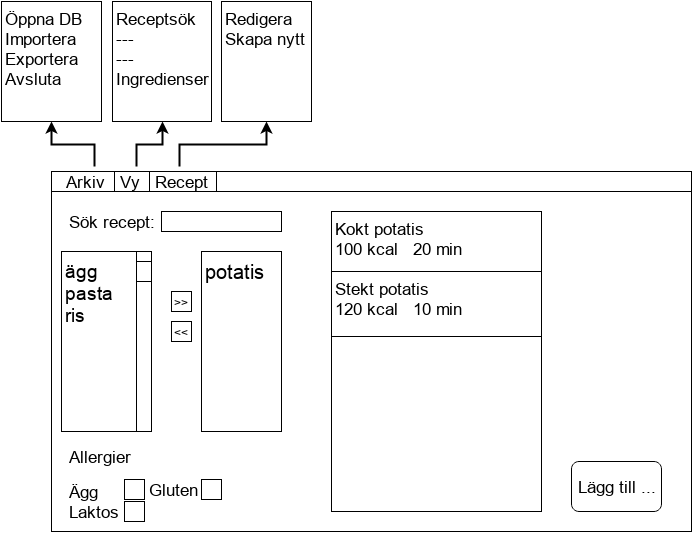
\includegraphics[scale=.5]{vy1.png}
  \label{fig:vy1}
  \caption{Sökfönster}
\end{figure}

\begin{figure}[h]
  \centering
  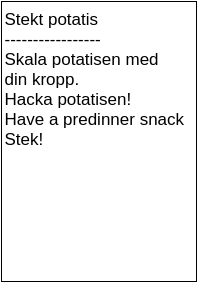
\includegraphics[scale=.5]{vy2.png}
  \label{fig:vy2}
  \caption{Receptfönster}
\end{figure}

\begin{figure}[h]
  \centering
  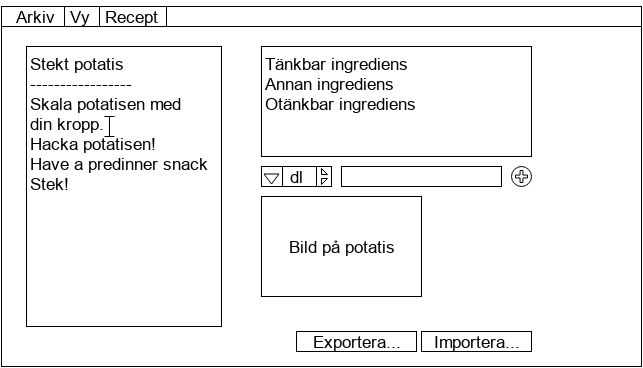
\includegraphics[scale=.5]{vy3.png}
  \label{fig:vy3}
  \caption{Redigering av recept}
\end{figure}

\begin{figure}[h]
  \centering
  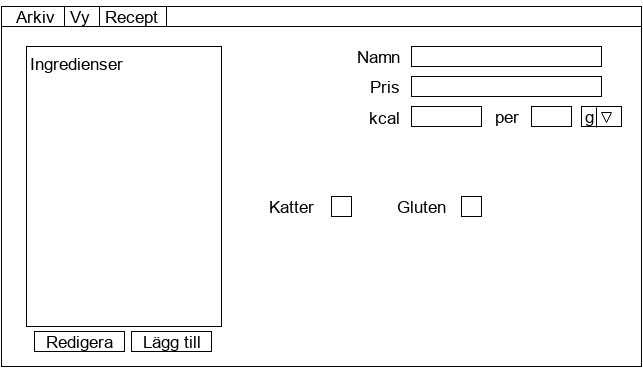
\includegraphics[scale=.5]{vy4.png}
  \label{fig:vy4}
  \caption{Redigering av ingredienser}
\end{figure}


\section{Databasen}
Databasen skall inehålla två entiteter recept och ingredienser recept skall ha fält för namn, betyg och en lista över vilka ingredienser som ingår och i vilket antal. Ingredienserna skall ha fält för pris, energiinnehåll och allergener.


\end{document}
